% Figure 6: Graceful Degradation Curves
\documentclass[tikz,border=5pt]{standalone}
\usepackage{pgfplots}
\pgfplotsset{compat=1.18}

\begin{document}
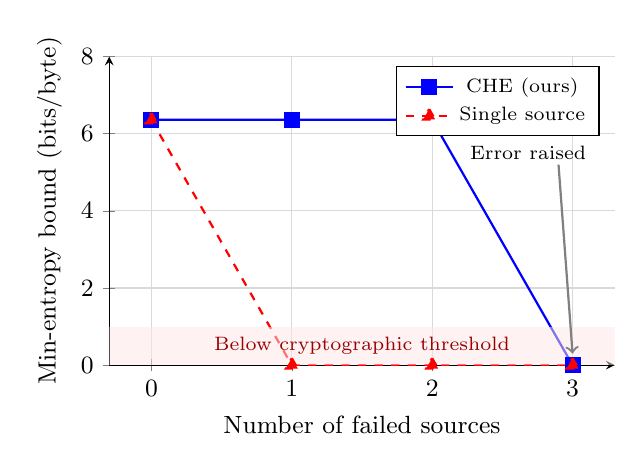
\begin{tikzpicture}
\begin{axis}[
  width=8cm, height=5.5cm,
  xlabel={Number of failed sources},
  ylabel={Min-entropy bound (bits/byte)},
  xmin=-0.3, xmax=3.3,
  ymin=0, ymax=8,
  xtick={0,1,2,3},
  ytick={0,2,4,6,8},
  grid=major,
  grid style={gray!30},
  legend pos=north east,
  legend style={font=\scriptsize},
  axis lines=left,
  font=\small,
]

% CHE graceful degradation
\addplot[thick, blue, mark=square*, mark size=2.5pt] coordinates {
  (0, 6.36)
  (1, 6.36)
  (2, 6.36)
  (3, 0)
};
\addlegendentry{CHE (ours)}

% Naive single-source (cliff drop)
\addplot[thick, red, dashed, mark=triangle*, mark size=2.5pt] coordinates {
  (0, 6.36)
  (1, 0)
  (2, 0)
  (3, 0)
};
\addlegendentry{Single source}

% Unsafe zone
\fill[red!10, opacity=0.5] (axis cs:-0.3,0) rectangle (axis cs:3.3,1);
\node[font=\scriptsize, text=red!60!black] at (axis cs:1.5, 0.5) {Below cryptographic threshold};

% Error annotation
\node[font=\scriptsize, anchor=west] at (axis cs:2.2, 5.5) {Error raised};
\draw[->, gray, thick] (axis cs:2.9, 5.2) -- (axis cs:3, 0.3);

\end{axis}
\end{tikzpicture}
\end{document}
